\documentclass[a4paper]{article}

\usepackage[english]{babel}
\usepackage[utf8]{inputenc}
\usepackage{amsmath}
\DeclareMathOperator*{\argmax}{argmax}
\usepackage{graphicx}
\usepackage[colorinlistoftodos]{todonotes}
%\usepackage{hyperref}



\title{Final Year Project Progress Report}

\author{Samuel Lee}

\date{18 January 2019}

\begin{document}

\begin{titlepage}
	\begin{center}
		
		
\includegraphics[width=0.8\textwidth]{NTU.png}
		\vspace{2cm}
		
		\huge
		
		\textbf{Pricing problems with \\Thompson Sampling}
		
		\vspace{1cm}
		\Large
		Lee Wai Leong Samuel
		
		\vspace{2cm}
		\Large
		Nanyang Technological University\\
		School of Physical and Mathematical Sciences\\
		8 April 2019
		
		\vfill
		
		Final Year Project\\
		Supervisor: Dr. Yan Zhenzhen
		
		\vspace{0.8cm}
		
	\end{center}
\end{titlepage}

\begin{center}
	\renewcommand{\baselinestretch}{1.5}
	\large
	\textbf{Acknowledgements}
	\vspace{1cm}
	
	My heartfelt thanks and gratitude go to Dr. Yan Zhenzhen for her patience and guidance throughout the project. There were times when I felt lost and was on the verge of giving up but she has been extremely understanding and encouraging. I have learned and grown a lot both technically and personally from her knowledge and enthusiasm on this topic. It has been a great privilege to have her as my thesis supervisor.
\end{center}
\pagebreak
\begin{center}
	\renewcommand{\baselinestretch}{1.5}
	\large
	\textbf{Abstract}
	\vspace{1cm}
	
	
	In 1933, William R. Thompson proposed an algorithm known as Thompson sampling in order to maximise culmulative payoff in a multi-armed bandit (MAB) problem. MAB problems have been frequently used to model real-life decision making scenarios. This paper explores the extension of Thompson sampling to other problems beyond the MAB setting. More specifically, Thompson sampling is applied to product sales in a dynamic pricing setting as part of the multi-product pricing problem. 
\end{center}
\pagebreak
\large
\renewcommand{\baselinestretch}{1.5}
\tableofcontents



\pagebreak
\section{Introduction}
\subsection{Problem description}
With sales reaching 10\% of total global sales, there is little doubt that e-commerce is a very popular online activity \cite{nano3}. It is expected to continue growing to 15\% in 2020 which has led to many firms setting up their own e-commerce portals or through other e-commerce giants. In order to differentiate themselves from the competition, most firms implement some sort of sales promotion. Some examples of promotions include percentage discounts (X\% off), flat amount discounts (\$X dollars off), BOGO (Buy one get one at X\% off) which is commonly used to clear excess stock and multi-buys (2 for the price of 1). In this project, further study is conducted on full-cut promotions in a dynamic pricing problem. Dynamic pricing involves a seller regularly adjusting the prices of products in order to obtain information about the products' demand, and then exploiting this information in order to maximise revenue. In a ``full-cut promotion", there is usually a pre-determined amount. For each time an order satisfies the pre-determined amount, it would be eligible for a flat amount discount. For example, Calvin Klein recently had the promotion ``For every \$100 spent, enjoy \$40 off" on their website \cite{CK}. It would thus be valuable to study full-cut promotions as they are implemented very frequently in e-commerce. 
\subsection{Literature review}
In order to study full-cut promotions, the multi-product pricing problem should first be investigated as it is a more fundamental problem of dynamic pricing problems. In this area, work has been done in the cases of known demand function and unknown demand function. In the former case, the dynamic pricing problem is typically modelled as the multi-armed bandit (MAB) problem and is solved by well-known methods such as the upper confidence bound (UCB) algorithm. Bubeck \& Cesa-Bianchi (2012) summarised this problem without resource constraints in their paper. Badanidiyuru et al. (2013) further improved on this approach by adapting the UCB algorithm to a MAB problem with resource constraints as such constraints cannot be easily modelled in the typical MAB problem. This was achieved by maintaining a vector of costs and adjusting it by combining confidence bounds and multiplicative updates. 
\newline
\newline
In the latter case of unknown demand function, Aviv \& Pazgal (2005) used a certainty-equivalent heuristic to obtain an approximate pricing solution in a partially observed Markov decision process (POMDP) framework. Both Araman \& Caldentey (2009) and Farias \& Van Roy (2010) extended on this approach by proposing more sophisticated approximate dynamic programming heuristics. Araman \& Caldentey (2009) used a sequence of models with varying levels of complexity to model the demand in which the underlying process followed a Poisson distribution, and then proposed a set of algorithms that efficiently approximated the solution. Similarly, Farias \& Van Roy (2010) also used a Poisson distribution for their model but with a different heuristic approach which they called \textit{decay balancing.} Broder \& Rusmevichientong (2012) used maximum likelihood estimation to obtain pricing policies under a general parametric choice model and also when the family of demand functions satisfied a ``well-separated" condition. 
\newline
\newline
In this project, the objective is to apply Thompson sampling to solve the dynamic pricing problem in a MAB setting for sales under full-cut promotions. While many other efficient algorithms exist to solve MAB problems, Thompson sampling was chosen as it has been shown to be highly competitive with promising performance \cite{thomp}. 

\section{Understanding the data}
\label{sec:introduction}
The given data is sales data of 66 products sold over a period of 11 days without any changes in price while under some sales promotion from an e-commerce firm based in China. The dataset contained 4716 rows and 23 columns. Each row represented a product in an order that was placed while each column represented a feature of each order such as order ID, order date, user ID, goods ID, price and quantity.
\newline
\newline
It is known that there is an ongoing sales promotion in the data in which an order would be eligible for discounts by fulfilling a minimum value. This value is defined as the threshold. For example, every \$99 spent would be eligible for a \$50 discount. One possible method to find the threshold would be through trial and error.
\newline
\newline
If $X$ is trialed as the threshold value, orders can be categorized into groups of different multiples of $X$. The first group would consist of orders ranging from \$0 to \$($X$-1) and the second group would range from \$$X$ to \$2$X$-1 and so on. The mean discount for each group can then be calculated. If $X$ is the threshold value, the mean discount for the first group should be 0 as all orders in that group should not have fulfilled the minimum amount. Likewise, the mean discount for subsequent groups should be multiples of the discount. Plotting the mean discounts for each group should reveal a linear relationship.
\newline
\newline
For this data set, multiple values of $X$ (80, 90, 99, 110, 120) were tested and the mean discounts were plotted. For $X = 80, 110$ and $120$, the gradients are not constant over each group. This suggests that some groups contain orders that qualify for different discounts from the rest. The plots of $X = 90$ and $X = 99$ indicate a strong linear relationship. However, at $Groups = 3$, the plot of $X = 90$ is not as linear as $X=99$. Thus, it is likely that the true threshold value of this data set is 99.

\begin{figure}
	\centering
	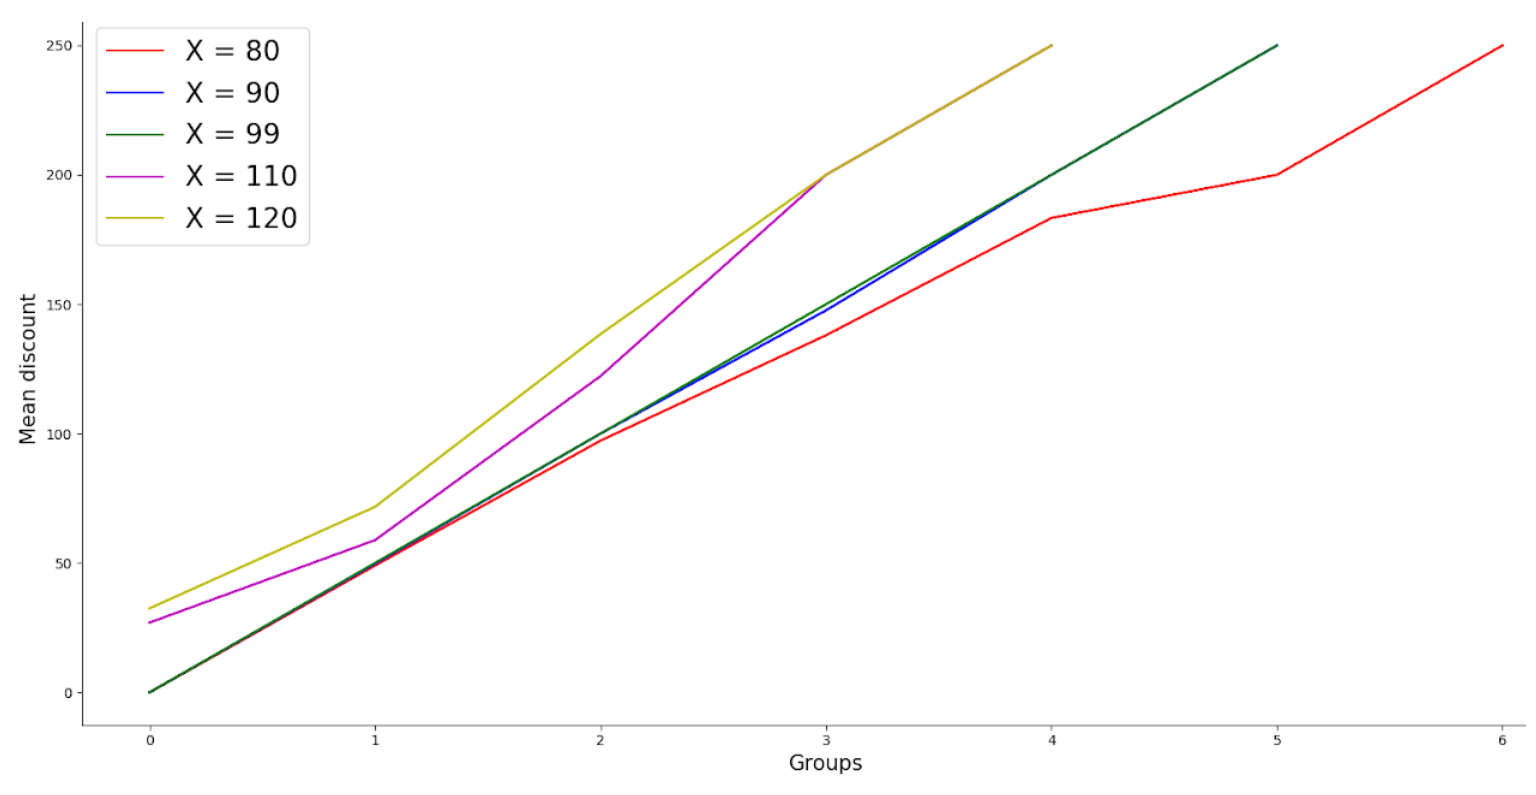
\includegraphics[width=1\textwidth]{cut.png}
	\caption{\label{fig:cut}Plotting mean discounts for each group}
\end{figure}
\section{Description of approaches}
\label{sec:approach}
The first approach would be to use the classical Thompson sampling algorithm in a MAB problem where each price vector represents an arm and the objective is to investigate which arm has the highest expected payout so as to maximize revenue over time. In this approach, there is a finite number of price vectors and the goal is to learn the demand distribution of each price vector.
\newline
\newline
The second approach would be to use Thompson sampling in a dynamic pricing algorithm. In this approach, there is usually a larger set (possibly infinite) of price vectors. The goal is to learn the distribution of the price elasticity of each product and not the distribution under each price vector.

\section{Generating training data}
\label{sec:theory}
Since the data set only contained sales data for one set of price, there is insufficient data to perform Thompson sampling. Thus, simulation data was created and the set of prices in the data set was used as one price vector. 
\newline
\newline
For each price vector $i$, a theoretical sales data was created using the formula below and it represents the true demand under this price vector.
\[X_i = \frac{e^{V_i - P_i}}{\sum_{j=0}^{N}e^{V_j - P_j}} \tag{1}\]
where $V_i$ represents the customer's valuation of product $i$ and $P_i$ is the price of product $i$. In the denominator, $j=0$ represents the option where the customer chooses not to buy anything. For the first approach, in addition to the original price vector, two other price vectors were created where the first vector is created by adding 5 to the original price vector and the second vector is created by subtracting 5 from the original price vector. The 3 price vectors may be identified as lower price vector, middle price vector and higher price vector.
\newline
\newline
As there are now 3 price vectors, the valuation vector $V$ can be created by randomly sampling from a 5\% neighbourhood of $\hat{P}$ where $\hat{P}=\sum_{k=1}^{3}P_k$. $V_0$ is randomly sampled from the interval $(0,5).$
\newline
\newline
With the $V$ and $P$ vectors defined, the theoretical $X_i$ corresponding to each price vector can be created and they will represent the true demand. In the long run, the expected value of all data points for each price vector should be equal to the theoretical $X_i$.
\newline
\newline
For each price vector, 20 data points were created. In order to ensure that the expected value of all data points was equal to the theoretical $X_i$, 10 epsilon vectors were created and the data points were obtained by adding and subtracting the epsilon vector from the theoretical $X_i$. This process was repeated for the other two price vectors as well. In total, there were 60 data points created with each price vector having 20 data points.

\section{First approach}
In this approach, the objective was to learn the true demand function under each price vector. It was assumed that the true demand functions followed normal distributions. The prior distribution for each price vector was then estimated from the 20 data points generated earlier using maximum likelihood estimation. 
\newline
\newline
For iterations $k = 1,...,K$, the following process was done. 
\begin{enumerate}
	\item A random sample was taken from each price vector's prior distribution.
	\item The estimated revenue under each price vector was calculated by multiplying the random sample and the price vector since each random sample represents the estimated demand under that price vector.
	\item The price vector with the highest estimated revenue was chosen as the selected arm for this iteration.
	\item The selected arm was pulled. The observed demand would be that price vector's theoretical $X_i$.
	\item The observed revenue was calculated by multiplying the observed demand with the price vector and also accumulated over all iterations.
	\item The observed demand was added as an observation to the selected arm's $H_{k-1}$ data points where $H_{k-1}$ is the number of data points under that price vector in the previous iteration.
	\item The prior distribution of that price vector was re-estimated using the $H_{k-1} + 1$ data points.
\end{enumerate}
\begin{figure}
	\centering
	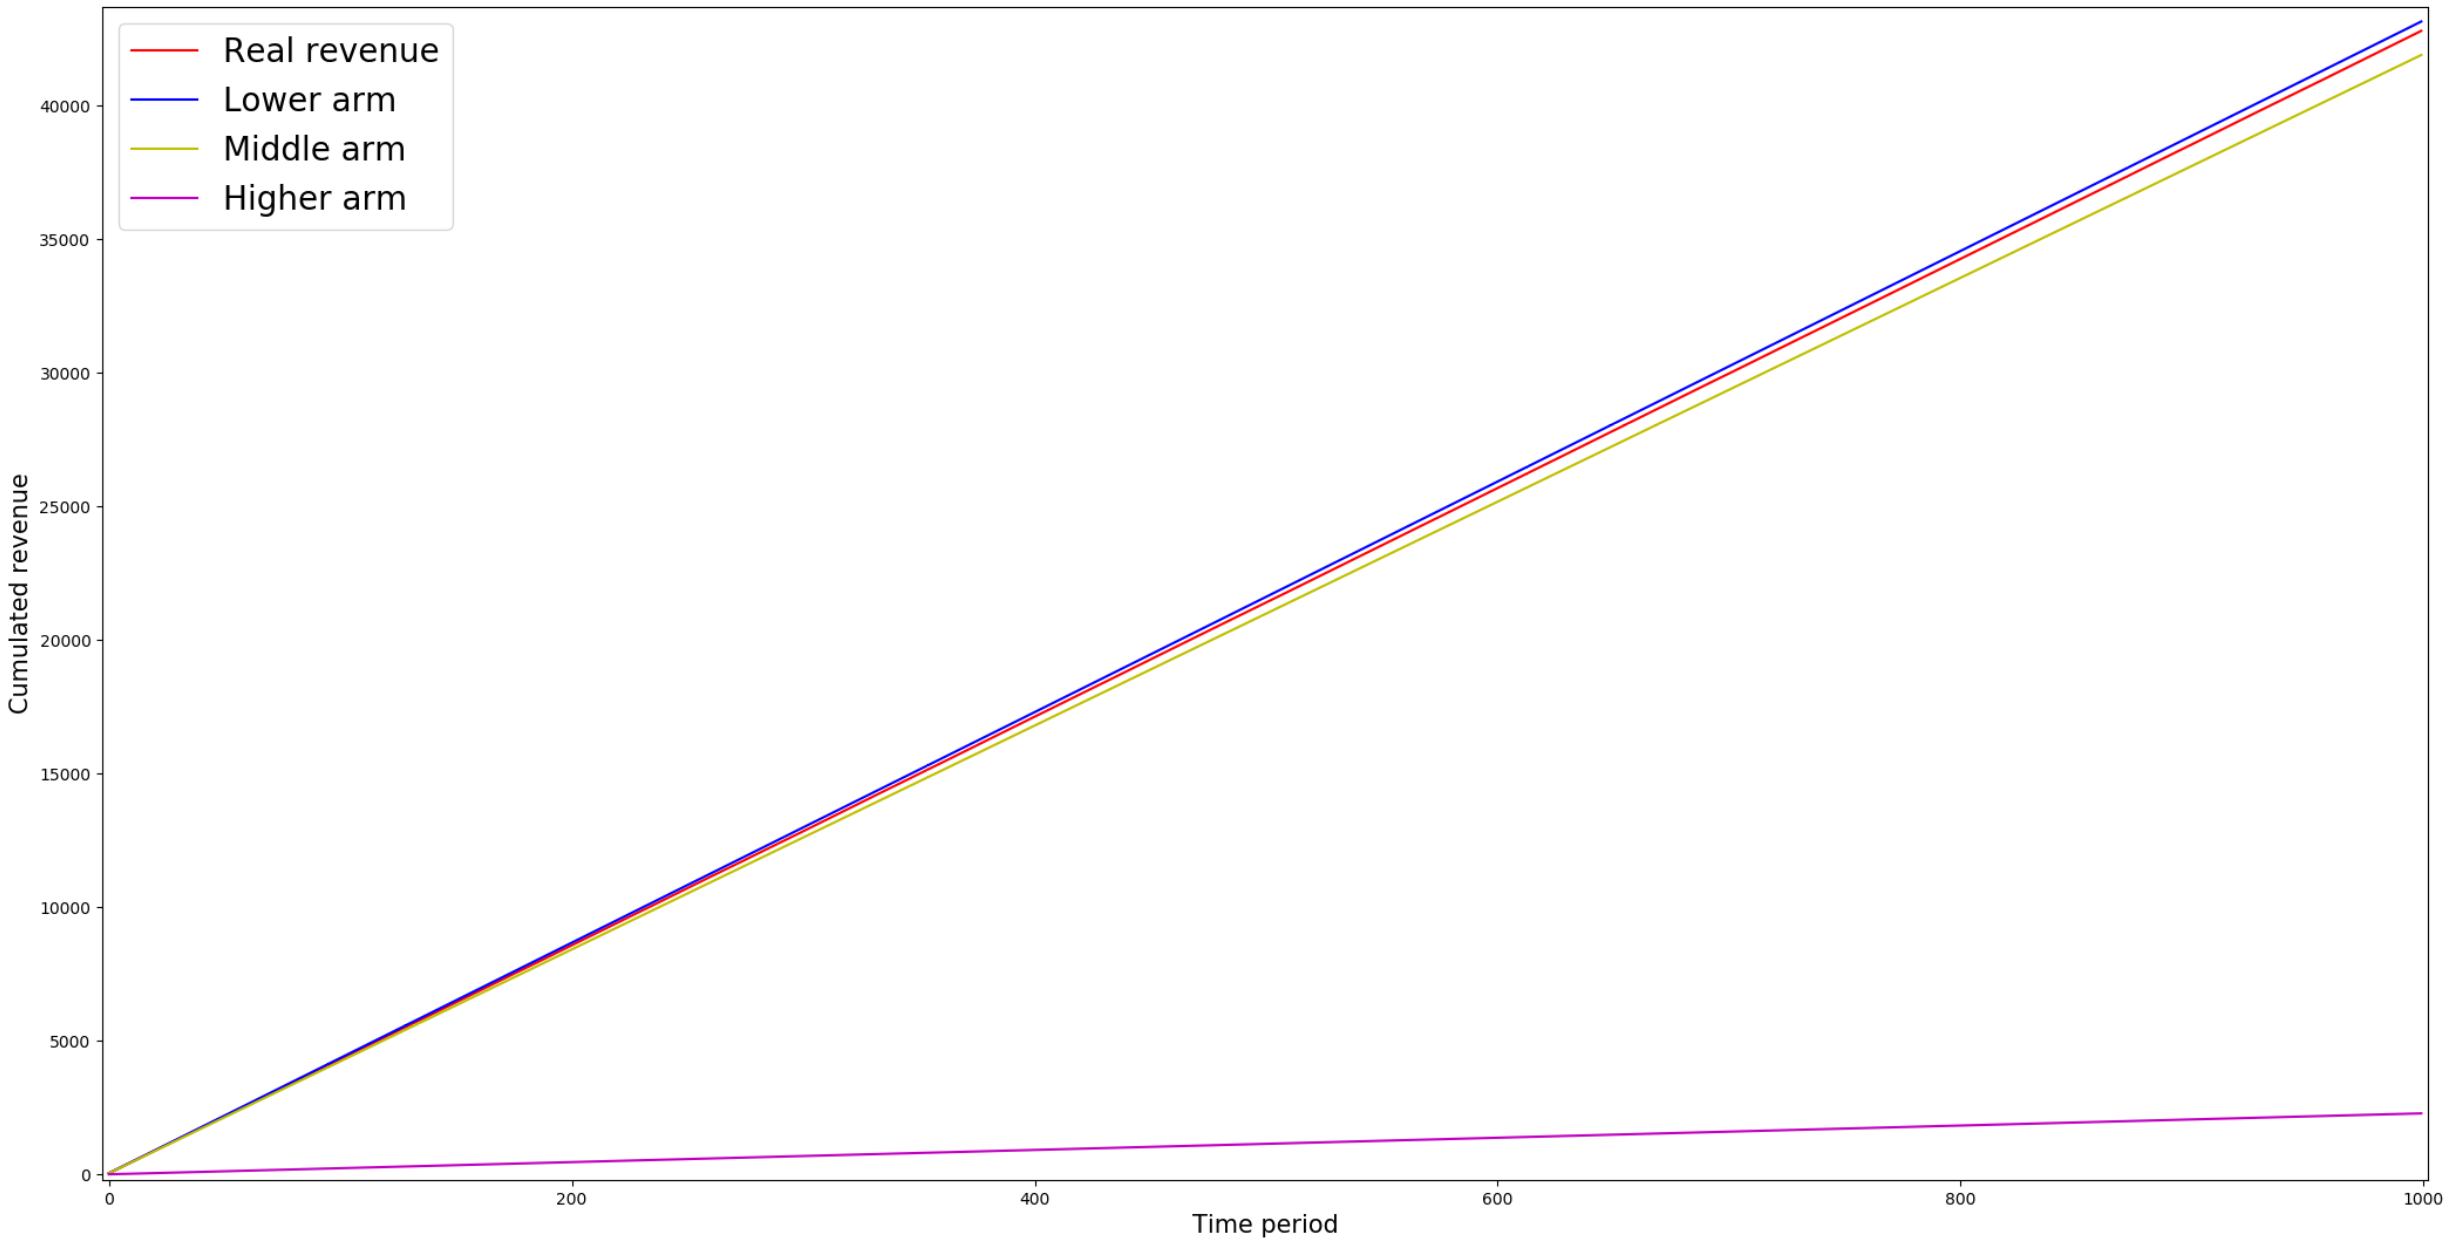
\includegraphics[width=1\textwidth]{approach1.png}
	\caption{\label{fig:one}Comparing revenue between all 3 arms and actual revenue}
\end{figure}
The number of times each price vector was selected was recorded. The price vector that was selected the most often would then be the arm with the highest revenue.
\newline
\newline
In order to validate that the chosen arm in the above process was the correct arm, a simple check was conducted for each arm. In each check, the same arm was chosen in every iteration and the observed revenue was cumulated. The arm with the greatest cumulated revenue would then be the theoretically correct arm. The result of one initialisation of this approach over 1000 iterations is shown in Figure 2.
\newline
\newline
The blue, yellow and purple plots correspond to checks for each arm and they represent the true revenue under that arm. Since the lower arm has the highest cumulated revenue, it is the theoretically correct arm. The red plot represents the revenue under this algorithm. It can be seen that the algorithm does not choose the higher arm at any time periods as its revenue is always between the lower and middle arm. As the time periods increase, there is a well-defined separation between the real revenue, lower and middle arm with the real revenue being closer to the lower arm. This is because the algorithm has already correctly identified the theoretically correct arm and was exploiting it in every iteration. 
\newline
\newline
Similarly, in other initialisations of this approach, the algorithm always correctly identifies the theoretically correct arm and maximises revenue over the time periods.


\section{Second approach}
In this approach, the objective was to learn the true elasticity values for each product. Since the order of prior data affects elasticity, it was assumed that the order of the price vectors implemented was as follows: lower price vector, original price vector, higher price vector. With this ordering, the prior estimates of the elasticity values could be obtained using the following formula
\[\gamma_i = \frac{\frac{x_{i,t+1}-x_{i,t}}{x_{i,t}}}{\frac{p_{i,t+1}-p_{i,t}}{p_{i,t}}}\]
where $\gamma_i$ is the elasticity of product $i$. It was assumed that the true elasticities followed a normal distribution i.e $\Pi_0(\gamma_*)=N(\mu_0,\Sigma_0)$. The prior estimates $\gamma_i$ were taken as the mean $\mu_0$ of the distribution while the covariance matrix was set as $\Sigma_0 = cI$. $c$ was set as $c = \frac{1}{10}\sum_{i=1}^{i=N}\gamma_i$
\newline
\newline
For iterations $k = 1,...,K$, the following process was done. 
\begin{enumerate}
	\item Randomly sampled from $\gamma_t \sim \Pi_{t-1}$ until all components of $\gamma_t$ are negative since elasticity values are negative.
	\item Forecasted demand $f_{i,t}$ of the following day using a vector autoregression model.
	\item Solved the following optimisation problem to get price vector $p_t$ given $p_{i,t-1}$ and estimates $f_{i,t}$ and $\gamma_t$ \[p_t = \argmax_p \sum_{i=1}^{N}\frac{p_i^2f_{i,t}\gamma_{*,i}}{p_{i,t-1}} -p_if_{i,t}\gamma_{*,i} + p_if_{i,t}\] \[\text{subject to: } p \in C_t \]
	\item Applied prices $p_t$. The observed demand would be generated by equation $(1)$ using $p_t$ and the same valuation vector $V$ in Section 3.
\end{enumerate}

\section{Timeline of future work}
Here is a timeline of how the project will progress in Semester 2 after the progress report has been submitted. 
\begin{itemize}
	\item Week 2 - 3, complete second approach
	\item Week 4 - 5, compare results of both approaches
	\item Week 6 - 9, application to full-cut promotion
	\item Week 10 - 11, compare numerical results with algorithms from other papers
	\item Week 12, complete final report for pre-examination
	\item Week 14, final presentation
	\item Week 15, submission of final report
\end{itemize}
\begin{thebibliography}{9}
	\bibitem{nano3}
	https://www.statista.com/statistics/534123/e-commerce-share-of-retail-sales-worldwide/
	
	\bibitem{CK}
	https://milled.com/CalvinKlein/final-hours-take-40-off-every-100-spent-Q2RTJAp7mfdfwq3I
	
	\bibitem{1}
	Araman, V. F., R. Caldentey. 2009. Dynamic pricing for nonperishable products with demand learning.
	\emph{Operations Research} 57(5) 1169-1188.
	
	\bibitem{1a}
	Aviv, Yossi and Pazgal, Amit. 2005. A partially observed markov decision process for dynamic
	pricing. \emph{Management Science} 51(9) 1400–1416.
	
	\bibitem{bada}
	Badanidiyuru, A., R. Kleinberg, A. Slivkins. 2013. Bandits with knapsacks. \emph{IEEE 54th Annual Symposium on Foundations of Computer Science (FOCS).} 207-216.	
	
	\bibitem{brod}
	Broder, Josef and Rusmevichientong, Paat. 2012. Dynamic pricing under a general parametric choice model. \emph{Operations Research} 60(4) 965-980.
	
	\bibitem{bub}
	Bubeck, S., N. Cesa-Bianchi. 2012. Regret analysis of stochastic and nonstochastic multi-armed bandit problems. \emph{Foundations and Trends in Machine Learning} 5(1) 1-122.
	
	\bibitem{thomp}
	Chapelle,  Li. 2011. An Empirical Evaluation of Thompson Sampling. NIPS. 
	
	\bibitem{2}
	Farias, V., B. Van Roy. 2010. Dynamic pricing with a prior on market response. \emph{Operations Research} 58(1) 16-29.
\end{thebibliography}

\end{document}